% !TEX root = ../report.tex

\clearpage
\chapter{Pattern Documentation}
\label{ch:patterns}


\section{Layers}
% see https://www.docker.com/sites/default/files/what-is-vm-diagram.png


\subsection{Client-Server}


\begin{figure}[H]
\centering
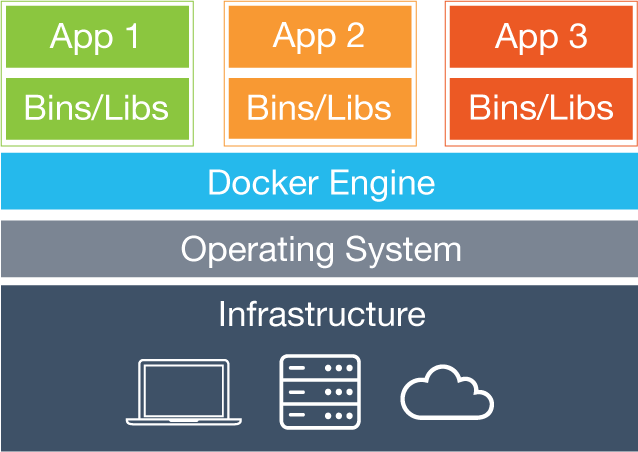
\includegraphics[scale=0.4]{5-patterns/images/what-is-vm-diagram.png}
\caption{A layered overview of the Docker. Source \cite{whatisdocker}}
\label{fig:layers-pattern}
\end{figure}

\begin{description}
\item [Traceability]~\\
The Layers pattern can be deducted from the online documentation\cite{dockerarchi}.

\item [Source]~\\
Architectural patterns revisited -- a pattern language, P. 29 \cite{avgeriou2005architectural}

\item [Issue]~\\
For a good encapsulation, each instance of docker is modeled using layers that interact with each other.

\item [Assumptions/Constraints]~\\
The interaction or communication between layers is carried out through socket, RESTful, or TCP/IP connection.

\item [Solution]~\\
Docker utilizes layers pattern. The system is modeled using layers and each component resides on a specific layer. An example can be seen in Figure \ref{fig:layers-pattern}.

\item [Rationale] ~\\
By separating each component in separated layers, the system will be more modular and have better security.

\item [Implications]~\\
There must be a clear closure of each layer. Communications protocol must also be defined.

\item [Related Patterns]~\\
\begin{itemize}
	\item Client-server
\end{itemize}
\end{description}

\clearpage
\section{Client-Server}

% see https://docs.docker.com/engine/introduction/understanding-docker/
% also nice image we can borrow: https://docs.docker.com/engine/article-img/architecture.svg
\begin{figure}[H]
\caption{An overview of the Docker architecture, showing the client and daemon. Source: \cite{dockerarchi}.}
\centering
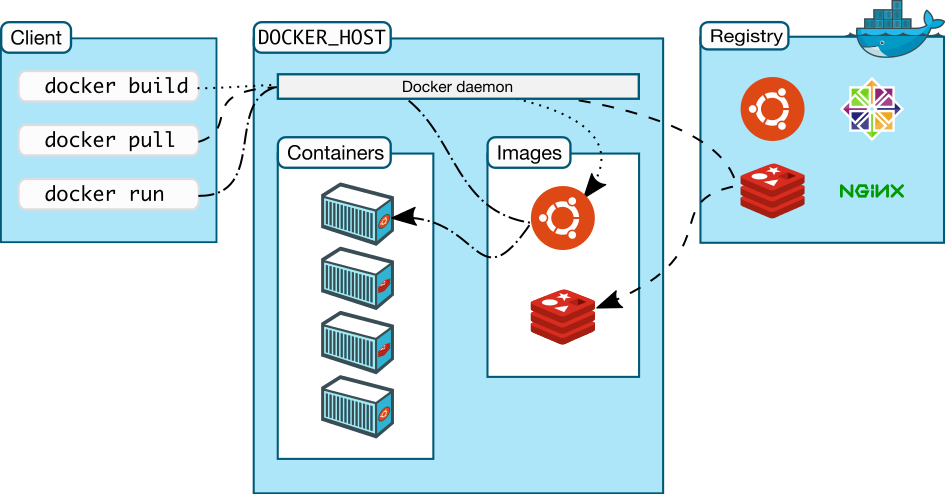
\includegraphics[scale=0.4]{4-softwarearch/images/architecture.png}
\end{figure}

\begin{description}
\item [Traceability]~\\


The Client-Server pattern can be deducted from the online documentation\cite{dockerarchi}.

The Client-Server pattern can be deducted from the `What is Docker’s architecture?' section of the online documentation\cite{dockerarchi}.

\item [Source]~\\
Architectural patterns revisited -- a pattern language, P. 29 \cite{avgeriou2005architectural}

\item [Issue]~\\


For good interoperability, it should be possible for Docker containers to be started remotely. A single interface should be able to control containers on numerous hosts.

\item [Assumptions/Constraints]~

\item [Solution]~\\
Docker uses a Client-Server architecture. The client, a binary supplying a command-line interface, act as the primary interface for the user. The user enters commands into this client, which are then send to a server: the docker daemon. 


It should be possible for Docker containers to be controlled remotely and a single interface should be able to control containers on multiple hosts (e.g. in the cloud).

Additionally, certain operating systems lack the underlying technologies necessary for running containers. For those OSes, it should be possible to call remote daemons running on operating systems which are supported. % /WindowsBashing
% Me wantz to run on da windooowz, butz it aint got no cgroups

\item [Assumptions/Constraints]~
\begin{itemize}
\item The versions of the client binary and the server binary should match. Different versions can cause problems.
\item All the services offered by the daemon have to be made available to the client using a REST interface.
\end{itemize}

\item [Solution]~\\
Docker uses a Client-Server architecture. The client, a binary supplying a command-line interface, act as the primary interface for the user. The user enters commands into this client, which are then sent to a server: the docker daemon. 


\item [Rationale] ~\\
The daemon is a background process, which supplies the requested services to the client. The daemon exposes a REST interface.

For Docker, the client can be configured to connect to other daemon processes than the one running on the local machine. It can be configured to connect to remote Docker daemons as well, allowing the user to issue commands to daemons running remotely.

%todo move above to architecture chapter 

By separating the client and server it is possible to use the same client to issue commands to different daemons, running on different hosts.
It is also possible to use the client on operating systems that do not support running containers.

\item [Implications]~\\
The use of the Client-Server pattern results in two different executable binaries: a daemon and a client. 


The use of a separated client handling the user interaction increases the modularity.
Furthermore, it increases the interoperability, since the client can send commands to daemons running on remote machines and the local machine.

All the services offered by the daemon have to be made available to the client using a REST interface.

It increases the interoperability, since the client can send commands to daemons running on remote machines and the local machine.

Additionally, the portability is increased, since the client can run on Operating System that cannot run containers themselves.


\item [Related Patterns]~\\


\end{description}


\section{Shared repository}
%\textit{Can we consider the docker registry a shared repository?}
% Schema
%http://fr.slideshare.net/Docker/https-dldropboxusercontentcomu20637798docker-meetup-freiburg
% http://blog.octo.com/en/docker-registry-first-steps/   http://fr.slideshare.net/egorpushkin/docker-demo   
% Because of Pull/¨Push can we talk about Pattern publish suscribe ?

The docker registry is considered as a Shared Repository. \\
Two alternatives exist:DockerHub and Docker Trusted Registry. \\

Docker has a feature wich can be configured : the Notification Sytem which makes the Shared Repository an active Repository.
\textit{https://docs.docker.com/registry/notifications/}

\begin{description}
\item[Traceability]~\\
The Shared Repository pattern can be deducted from the online documentation : \textit{https://docs.docker.com/registry/}
\quote{"The Registry is a stateless, highly scalable server side application that \textbf{stores} and lets you \textbf{distribute} Docker images. A registry is a storage and content delivery system."} 

\item[Source]~\\
%\EAA, P.322 \cite{eaa}\\
Architectural Pattern Revisited - A Pattern Language, P.13 \cite{avgeriou2005architectural}

\item[Issue]~\\
Docker provided a way for the user to store and distribute images.
User need to be alerted of new *** within the registry through notifications. % Develop ?

\item[Assumptions/ Contrainst]~\\

\item[Solution]~\\

\item[Rationale]~\\ % in which way this pattern helps Docker? What is the goal ?
By using the Shared Repository Pattern 


\end{description}


\section{Plugin}
%TODO image
\begin{description}

\item [Traceability]~\\
The existence of Docker Plugins becomes apparent from it's documentation at \cite{dockerplugindocs}.

Additionally, the directories \verb|docker/pkg/plugins/| \footnote{\url{https://github.com/docker/docker/tree/master/pkg/plugins}} and \verb|  docker/daemon/graphdriver/plugin.go| \footnote{\url{https://github.com/docker/docker/blob/master/daemon/graphdriver/plugin.go}} (among others) in the project's repository contain the code for discovering plugins and the interfaces the plugins should implement.

\item [Source]~\\
Patterns of Enterprise Application Architecture, P. 499 \cite{eaa}

\item [Issue]~\\
The users of Docker want to have customization, by extending Docker with third party custom-built tools. This customization means that third parties should be able to write plugins that extend Docker's core functionality.\cite{dockerpluginblog}

The implementation of such plugins is only available at runtime.

\item [Assumptions/Constraints]~
\begin{itemize}
\item Plugins can only extends the functionality of the components of Docker, that have an interface that plugins can implement.
\end{itemize}


\item [Solution]~\\
Docker uses the Plugin pattern to link the implementation of the interfaces of several extendable components with third-party implementation at runtime.

\item [Rationale] ~\\ % https://docs.docker.com/engine/extend/plugin_api/
Docker discovers plugins by looking for .sock, .spec or .json files in the plugin directories on the host system. These files describe how Docker can communicate with the plugins using the REST API (usually via a Unix socket).



The plugins themselves run as seperate processes on the same host as the Docker daemon and implement an HTTP server listening for requests from the Docker daemon. After a user requires a plugin (this is indicated e.g. as a command-line parameter when starting a container using the Docker client) Docker uses the discovery algorithm (See XXX process view). After that, Docker sends a handshake to the plugin and the plugin returns a list of which subsystems this plugin implements.  %TODO the process view


The plugins themselves run as separate processes on the same host as the Docker daemon and implement an HTTP server listening for requests from the Docker daemon. After a user requires a plugin (this is indicated e.g. as a command-line parameter when starting a container using the Docker client) Docker uses the discovery algorithm (See XXX process view). After that, Docker sends a handshake to the plugin and the plugin returns a list of which subsystems this plugin implements.


For these subsytems Docker will replace the default implementation by a Proxy, that forwards all calls over the REST interface to the plugin process.

\item [Implications]~\\
The use of the Plugins pattern means that the adaptability increases. 

\item [Related Patterns]~
\begin{itemize}
\item Proxy
\end{itemize}

\end{description}

